%%%%%%%%%%%%%%%%%%%%%%%%%%%%%%%%%%%%%%%%%%%%%%%%%%%%%%%%%%%%%%%%%%%%%%%%%%%%%%%%%%%%%
% MARKOV DECISION PROCESSES
%
% Introduction to MDPs, finite MDPs, infinite MDPs
% Semi MDPs
% Partially Observable MDPs
%
%%%%%%%%%%%%%%%%%%%%%%%%%%%%%%%%%%%%%%%%%%%%%%%%%%%%%%%%%%%%%%%%%%%%%%%%%%%%%%%%%%%%%

\section{Markov Decision Processes}
In the face of uncertainty, the agent's \textit{sequential} decision making is formalized in the Markov decision process (MDP). The general MDP framework is shown in Figure \ref{fig:01mdp} and contains two components: the \textbf{agent} and the \textbf{system}. The \textbf{agent} is a continuously learning decision maker and is mathematically represented by the RL algorithm. Objectively, the agent will undergo numerous meaningful interactions with the system to ultimately learn the optimal policy, $\pi^*$ (i.e., the optimal decisions given different situations). Conversely, the \textbf{system} contains all elements the agent cannot arbitrarily control. In process control, the ambient temperature, actuators, and even the wires transporting the control signals are all part of the system because the agent cannot \textit{deterministically} manipulate them. 

\begin{figure}[H]
    \centering
    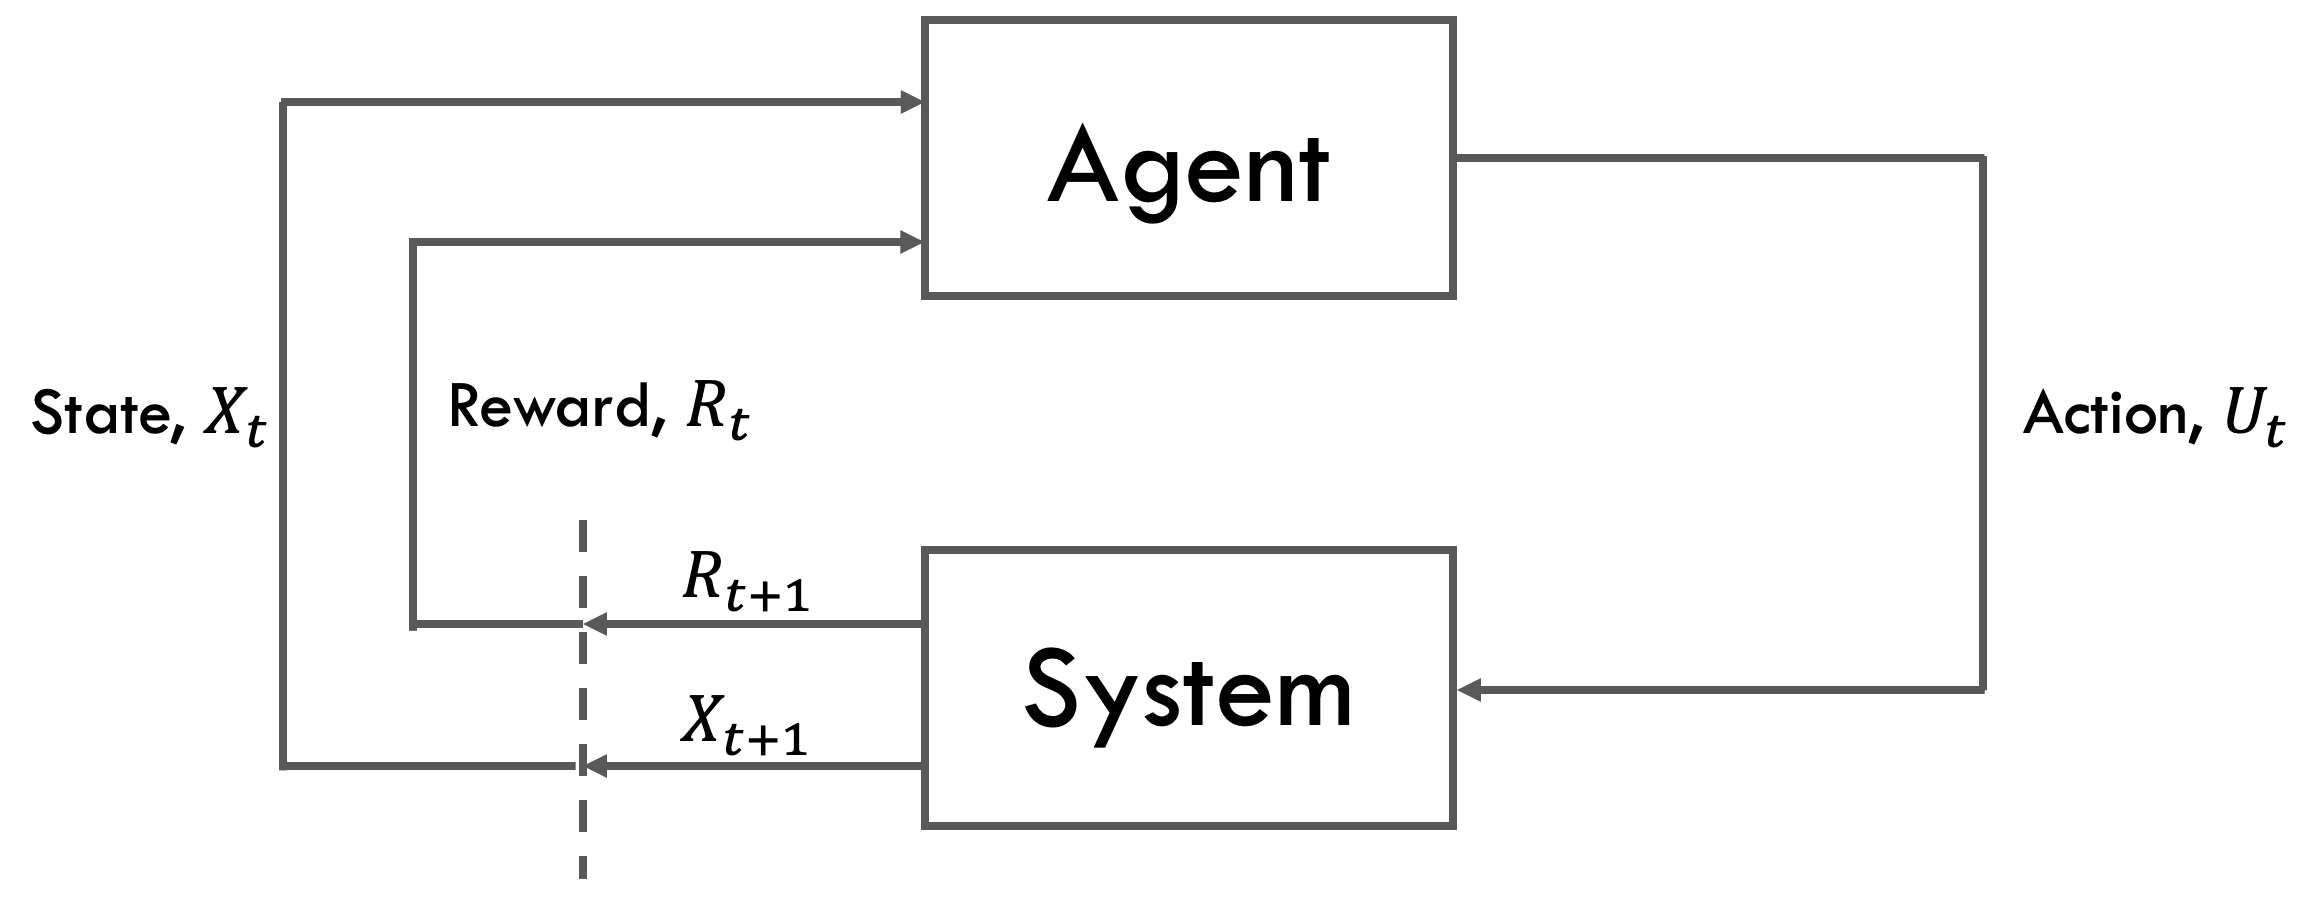
\includegraphics[width=0.56\textwidth]{images/ch1/MDP.jpeg}
    \caption{The general Markov decision process framework. Original image from \cite{sutton}.}
    \label{fig:01mdp}
\end{figure}   

Mathematically, the MDP is a discrete representation of the stochastic optimal problem and a classical formulation of \textit{sequential} decision making where both the immediate and long term consequences are explicitly considered \cite{bellman1, mdp_bellman}. Many definitions of the MDP exist and are equivalent up to small alterations of the process.  One comprehensive definition is that a MDP is a tuple $\mathcal{M}$, is a tuple $(\mathcal{X}, \mathcal{U}$, $P(x', r|x, u), \gamma, R)$ comprised of the following\cite{ng_ref12}:
\begin{itemize}
    \item $x \in \mathcal{X}$: \textbf{State} space of the system at each time step. Common states in industrial processes include temperatures, valve positions, pressures, flow rates, etc.
    \item $u \in \mathcal{U}$: Bounded \textbf{action} space of the agent, ($\mathcal{U}$ $ \geq 2 $). In traditional control, this is the \textbf{bounded input signals} sent to the actuators.
    \item $R \in \mathbb{R}$: Expected \textbf{reward} signal after performing action $u$ in state $x$. Reward functions are designed based on a desired performance metric.  In control theory, the reward function is known as the \textbf{objective function}.  Typically, $|R| \leq \mathcal{R}$ for convergence guarantees.
    \item $p(x', r|x, u)$: Systems \textbf{dynamics function}. Formally, it is the probability of transitioning to $x'$ and receiving $r$,  given states $x \in \mathcal{X}$ and performing action $u \in \mathcal{U}$. Mathematically, it is described by the following:
    \begin{equation}
        p(x', r | x, u) \dot{=} Pr\{X_t = x', R_t = r | X_{t - 1} = x, U_{t-1} = u\}
        \label{eq:transition_prob}
    \end{equation}
    where $p$ describes the system \textbf{dynamics} and $Pr$ denotes the probability operation \cite{sutton}. Additionally, $p$ satisfies the following equality:
    \begin{equation}
        \sum\limits_{x' \in \mathcal{X}} \sum\limits_{r \in \mathcal{R}} p(x', r | x, u) = 1, \forall x \in \mathcal{X}, u \in \mathcal{U}
        \label{eq:prob}
    \end{equation}
    Notice here that $p$ is only a function of the \textit{immediate past}, thus assuming that $x_{t - 1}$ and $u_{t-1}$ captures the complete history. This is known as the Markov property and its underlining assumptions are critical for successful process control applications using RL. Additionally, note that when the state and actions are formulated as augmented past information: $x_{t-1} = [s_{t-1}, s_{t-2}, ... s_{t-N}], u_{t-1} = [a_{t-1}, a_{t-2}, ..., a_{t-N}]$, where $s_{t-N}$ and $a_{t-N}$ denotes the past states and actions, the system is still Markov because decisions can be made exclusively using $x_{t-1}$ and $u_{t-1}$. 
    \item $\gamma$: \textbf{Discount factor} associated with uncertainty of the future, ($0 \leq \gamma \leq 1)$. $\gamma < 1$ is also a requirement for continuous processes to guarantee eventual convergence.
\end{itemize}

There exists three different MDPs: fully observable MDP (FOMDP), partially observable MDP (POMDP), and semi MDP (SMDP). Table \ref{tab:01mdps} shows a general guideline on the different MDPs.

\begin{table}[H]
\caption{A comparison of different Markov decision processes.}
\centering
\begin{tabular}{c|c|c}
\textbf{FO-MDPs}	& \textbf{S-MDPs}	& \textbf{PO-MDPs}\\
\hline
All states observable		  & All states observable			& Some states observable \\
Discrete time		          & Continuous time	             	& Discrete time \\
\end{tabular}
\label{tab:01mdps}
\end{table}

\subsection{Fully observable Markov decision processes}
Fully observable Markov decision processes are the simplest and serves as the foundational framework.  They are mainly applied to discrete systems with fixed sampling times where transition dynamics are unimportant and all states are observable (measurable in control literature). Here, the agent starts in some initial states, $x_0$. At each time $t$, the agent maps $x_t$ to some $u_t$ corresponding to its policy, $\pi_t$.  Given $x_t$ and $u_t$, the system will then transition to some new states $x_{t+1}$ dictated by Equation \ref{eq:transition_prob} while outputting reward signal $R_{t+1}$ based on the reward function. In regulation and set-point tracking problems, this reward function is typically the squared tracking error between $x_t$ and $x_{sp}$.  By repeating this cycle many times, the agent is able to traverse through some sequence, $x_t, u_t, R_{t+1}, x_{t+1}, u_{t+1}, R_{t+2}, x_{t+3}, ...$ and accumulate \cite{sutton}:
\begin{align}
G_t &= R_{t+1} + \gamma R_{t+2} + \gamma^2 R_{t+3} ... \\
    &= \sum\limits^{\infty}_{k = 0} \gamma^k R_{t+k+1}
\label{eq:return}
\end{align}
where $G_t$ denotes the cumulative discounted return at time $t$ and $\gamma$ is the discount factor to capture the future uncertainty. MDPs can represent both finite or infinite systems; the former describes episodic tasks with explicit terminal states while the latter describes tasks that continue forever.  Intuitively, most two-player board games such as Checkers, Chess, or Go are finite MDPs where the game is terminated after one player is defeated.  Contrarily, an infinite MDP system could be the control system in an industrial process. For infinite MDP systems, $\gamma < 1$ is a necessary condition to keep $G_t$ bounded. Ultimately, the agent is tasked with finding the optimal policy, $\pi^*$, that maximize $G_t$, and subsequently the value function, over $N$ steps. The value function for each state is given as \cite{sutton}:
\begin{align}
    v_\pi (x) &\dot{=} \mathbb{E}_\pi [G_t | X_t = x] \\
              &= \mathbb{E}_\pi \left[\sum\limits^\infty_{k=0} \gamma^k R_{t+k+1} | X_t = x \right] \\
              &= \mathbb{E}_\pi [R_{t+1} + \gamma G_{t+1} | X_t = x]
    \label{eq:value_func}
\end{align}
where $v_\pi (x)$ is the value function of $x$ under policy $\pi$. Theoretically, the existence and uniqueness of $v_{\pi}$ is guaranteed for continuous systems where $\gamma < 1$ or in systems with guaranteed termination.  Compared to Equation \ref{eq:01value}, Equation \ref{eq:value_func} takes the expectation of $G_t$; therefore, explicitly optimizing the long term returns rather than only the immediate rewards. The action-value formulation of Equation \ref{eq:value_func} is:
\begin{align}
    q_\pi (x, u) \; &\dot{=} \; \mathbb{E}_\pi [G_t | X_t = x, U_t = u] \\
                 &= \mathbb{E}_\pi \left[\sum\limits^\infty_{k=0} \gamma^k R_{t+k+1} | X_t = x, U_t = u \right], \forall x, u \in \mathcal{X, U}
    \label{eq:a_value_func}
\end{align}
FOMDPs work well for discrete systems where all states are observable.  However, system states in industrial processes are often unobservable (unmeasurable in control) due to limited hardware or engineering limitations. In such systems, the Markov property no longer holds resulting in sub-optimal decision making of the agent.





\subsection{Partially observable Markov decision processes}
Partially observable Markov decision processes (POMDPs) extend upon the concepts of FOMDPs and represent systems with unobservable states. In RL literature, observability is equivalent to measurability in control; thus, the two terms are used interchangeably here-forth. In FOMDPs, the current state $x_t$ at each time $t$ is fully observable. In the more general setting of POMDPs, the entire state vector describing the agent's current situation is no longer available. Instead, the agent only has access to a set of possible observations $\mathcal{O}$. At each time $t$, the agent sees observation $o_t$ which correspond to probability distributions over states.  Using $o_t$, the agent can infer the states it \textit{might} currently be in \cite{ng_ref12}. Relating to a process control setting, existing sensors typically only measure a subset of the current states; however, by using available measurements, one can infer the remaining unmeasurable states using probabilistic approaches.

Generally, finding $\pi^*$ in a POMDP setting is significantly harder compared to FOMDPs.  Even finding a near-optimal policy is at least NP-hard (non-deterministic polynomial time) \cite{pomdp_time}.  Furthermore, even agents with access to all the system's true value functions are unable to behave optimally in a POMDP setting because the current states are unknown \cite{ng_ref12}. 

Belief states is one method for agents to behave optimally in POMDPs. On a high level, belief states transform the POMDP setting into its FOMDP counterpart through a probabilistic approach. Specifically, belief states, $b$, are probability distributions over states deduced using previous observations and actions. The probability distributions represent what the agent thinks its current state is. Using these probabilities, the agent can compute scalar value functions of each state-action pair and use these to act "optimally".  Note here that the agent's behaviour is optimal given the available information, and not optimal with respect to the system. An quantitative example is provided below:
\begin{quote}
    Suppose an agent exists in a two-input two-output (TITO) POMDP setting with two unobservable states ($x_1$ and $x_2$) and two actions ($u_1$ and $u_2$) and suppose the problem is only concerned with the immediate consequences (for longer horizons, the agent must also consider the long term rewards, making the example less intuitive). In this system, there are four value functions, one for each state-action pair. Suppose $u_1$ earns a reward of 2 in $x_1$ and 0 in $x_2$.  Similarily, $u_2$ earns a reward of 0 in $x_1$ and 1 in $x_2$.  Given $b_t = [0.2, 0.8]$ (probabilities of being in $x_1$ and $x_2$, respectively), then $Q(b_t, u_1) = 0.2 \cdot 2 + 0.8 \cdot 0 = 0.4$ and $Q(b_t, u_2) = 0.2 \cdot 0 + 0.8 \cdot 1 = 0.8$, resulting in $u_2$ being the optimal action.
\end{quote}

In control theory, observers, such as soft sensors, are used to estimate unmeasurable states.  Observers are typically $1^{st}$ principles, data driven, or probabilistic models. The concept of belief states is very similar to observer design in control theory. Traditionally, Kalman filter is a widely used observer design. Conversely, recurrent neural networks (RNNs) are widely used for belief state estimation in RL. The performance of RNN was compared with Kalman filter in \cite{RNNvsKF}, drawing similarities of the two methods' objective, theory, and performance.

System representations using FOMDPs and POMDPs work well in discrete tasks where transition times are constant and transition dynamics are disregarded; however, both topics are paramount for continuous optimal control.  







\subsection{Semi Markov decision processes}
Typical MDPs are discrete representations of the optimal control problem and are sub-optimal in continuous tasks. Semi-Markov decision processes (SMDP) are an extension of MDPs to continuing tasks with unknown transition times and system dynamics. In SMDPs, the transition dynamics of the system are explicitly captured using reward function \cite{continuous_rl_ref14}:
\begin{equation}
R(x_t, x_{t+1}, u_t) = \int\limits^\infty_0 \int\limits^t_0 e^{-\beta s} \rho(x_t, \pi (x_t))dsdF_{x_t, x_{t+1}}(t | \pi (x_t))
\label{eq:reward_rate}    
\end{equation}
where $R(x_t, x_{t+1}, u_t)$ is the expected reward to be received when transitioning from $x_t$ to $x_{t+1}$ after action $u_t$. The rewards, $R$, are calculated at each time step in the transition period to explicitly capture transition information. Then, the average reward of the transition is used to update the agent. Here, $\rho(x_t, \pi(x_t))$ represents the average reward during the transition following policy, $\pi$. $F_{x, x_{t+1}}(t, u)$ denotes the probability distribution of the time required to transition from $x_t$ to $x_{t+1}$.  Finally, $\beta > 0$ denotes the \textit{constant} discount factor in SMDPs, where higher $\beta$ results in short-sighted agents. In SMDPs, the discount factor is corrected for transition time during each update step.  The corrected discount factor is given by:
\begin{equation}
    \gamma(x_t, x_{t+1}, u) = \int\limits^{\infty}_0 e^{-\beta t} dF_{x_t, x_{t+1}}(t | \pi_t)
\end{equation}
where $\gamma (x_t, x_{t+1}, u_t)$ is the expected discount factor that will be applied to the value of state $x_{t+1}$ during the update step shown in Equation \ref{eq:bellman_eq}. The value function for SMDPs is obtained from combining Equations \ref{eq:reward_rate} and \ref{eq:value_func}:
\begin{equation}
v_{\pi}(x_t) = \frac{1 - e^{-\beta \tau}}{\beta} R(x_t, x_{t+1}, \pi(x_t)) + e^{-\beta \tau}v_{\pi}(x_{t+1})
\end{equation}
where $\tau$ is the unknown transition time.  Similarily, the action-value form is given by:
\begin{equation}
    q_{\pi}(x_t, u_t) = \frac{1 - e^{-\beta \tau}}{\beta} R(x_t, x_{t+1}, \pi(x_t)) + e^{-\beta \tau}  q_{\pi}(x_{t+1}, u_{t+1})
\end{equation}
By representing control problems as SMDPs, control strategies resulting in large overshoot, inverse response, or any other undesirable dynamics behaviour can be minimized. Additionally, the system will be able to handle systems with unknown transition times.  An intuitive example illustrating the advantages of SMDPs in process control is as follows:

\begin{quote}
    Suppose a refinery company is operating a continuously stirred tank reactor (CSTR). Objectively, the CSTR must maintain 200$^{\circ}$ C for optimal performance.  The temperature is controlled through a heat exchanger using cold water.  A RL agent was built to optimally control the flow of cold water to maintain the temperature set point. Suppose the CSTR starts at 220$^{\circ}$ C.  Agents using MDP representations may be overly aggressive and send large input signals because the reward is only calculated \textit{right before} the next evaluation step. Therefore, input signals resulting in large overshoot or inverse response may not be reflected in the reward. Contrarily, SMDP representation uses the average reward accumulated along the trajectory to provide feedback to the agent, allowing the transition dynamics to be explicitly captured. This way, input signals resulting in undesirable behaviour can be captured and mitigated. Furthermore, SMDP representations can have flexible evaluation times (traditional representations evaluate after a set time period), enabling re-evaluation during the transitional period and adjusts the discount factor in accordance to the elapsed time from last evaluation.
\end{quote}









\subsection{Optimal solution of the Markov decision processes}
The optimal solution to the RL problem refers to identifying a policy that generates the highest long term returns. Such a policy may not be unique; there may exist many optimal policies, where $v_{\pi^*_1} = v_{\pi^*_2} = ... = v_{\pi^*_N}$.  Formally, the optimal policy must satisfy the \textbf{principle of optimality}: the optimal policy $\pi^*$ is optimal if and only if $v_{\pi^*}(x) \geq v_{\pi \neq \pi^*}(x)$ for all $x \in \mathcal{X}$ \cite{PO}. Mathematically, the optimal value function is:
\begin{equation}
    v^*(x) \dot{=} \argmax_{\pi} v_{\pi}(x), \forall x \in \mathcal{X}
\end{equation}
with its action-value variant being:
\begin{equation}
    q^*(x, u) \dot{=} \argmax_{\pi} q_{\pi}(x, u), \forall x, u \in \mathcal{X, U}
\end{equation}
In a more explicit form, the optimal value function and action-value function written in terms of Equations \ref{eq:value_func} and \ref{eq:a_value_func} are given, respectively, by \cite{sutton}:
\begin{equation}
    v^*(x) = \argmax_{u} \mathbb{E}[R_{t+1} + \gamma v^*(X_{t+1}) | X_t = x, U_t = u]
    \label{eq:01valuefunc}
\end{equation}
\begin{equation}
    q^*(x, u) = \mathbb{E}\left[R_{t+1} + \gamma \argmax_{u_{t+1}} q^*(X_{t+1}, u_{t+1}) | X_t = x, U_t = u \right]
\end{equation}
Here, the $max$ operation denotes that the optimal action will be taken for the remaining of the trajectory. Theoretically, all optimal value functions can be explicitly solved using Equation \ref{eq:01valuefunc}; however, such a task would require unreasonable amounts of computation power for even simple systems. In the following section, three popular methods will be introduced to estimate the value and action-value functions in reinforcement learning.
